\documentclass{article}

\usepackage[utf8]{inputenc}
\usepackage[T1]{fontenc}
\usepackage{lipsum}
\usepackage{graphicx}
\usepackage{amsmath}
\usepackage[margin=1in]{geometry}
\usepackage{titlesec}
\usepackage{enumitem}

\titleformat{\section} 
{\LARGE\bfseries}{\thesection}{1em}{}

\titleformat{\subsection} 
{\Large\bfseries}{\thesection}{1em}{}

\begin{document}

\pagestyle{empty}

\section*{MySQL} 
\large

\textbf{MySQL} è un DBMS basato sul modello relazionale (\textit{RDBMS}). Supporta gran parte dei costrutti del linguaggio \textit{SQL 2.0} con viste, query annidate, vincoli di chiave, trigger e viste aggiornabili. Supporta anche l'esecuzione di \textbf{transazioni} su un tipo particolare di tabelle, dette \textbf{INNODB}. Inoltre supporta anche molte tipologie di dati numerici, testuali, temporali e binari. Per concludere, dispone di un proprio \textbf{linguaggio di estensione procedurale} per definire le \textbf{stored procedures}.\vspace{14pt}\\
MySQL \textbf{non} ha limiti espliciti sulla \textbf{dimensione massima} di un database e sul numero di tabelle. Il \textbf{numero massimo di righe} in una tabella \textbf{dipende dai vincoli imposti dal sistema operativo} sulla dimensione massima di un file.\\
Non esistono problemi dal punto di vista della concorrenza in termini di \textbf{numero massimo di connessioni simultanee} al server MySQL. Tuttavia, i problemi emergono dal punto di vista delle \textbf{risorse}, per cui il numero effettivo di connessioni simultanee supportate dipende dalle capacità e dalle risorse hardware dell’elaboratore. Si osservino ora diversi comandi.\vspace{14pt}\\
Per \textbf{creare un nuovo database}:
\begin{itemize}[label={ }, leftmargin=1cm]
    \item \textit{CREATE DATABASE [IF NOT EXIST] nomedb;}
\end{itemize}
Per \textbf{rimuovere un database}:
\begin{itemize}[label={ }, leftmargin=1cm]
    \item \textit{DROP DATABASE [IF EXIST] nomedb;}
\end{itemize}
Per vedere quali \textbf{db sono presenti} nel sistema:
\begin{itemize}[label={ }, leftmargin=1cm]
    \item \textit{SHOW databases;}
\end{itemize}
Per impostare il \textbf{db corrente}:
\begin{itemize}[label={ }, leftmargin=1cm]
    \item \textit{USE nomedatabase;}
\end{itemize}
Per \textbf{creare} una tabella:
\begin{itemize}[label={ }, leftmargin=1cm]
    \item \textit{CREATE [TEMPORARY] TABLE}
    \item \textit{nometabella | nomedb.nometabella}
    \item \textit{[definizione attributi]}
    \item \textit{[opzioni]}
    \item \textit{[select]}
\end{itemize}
E' possibile generare una tabella valida solo per la \textbf{sessione corrente} con l'opzione \textit{TEMPORARY}.\\
Inoltre è possibile \textbf{popolare} la tabella con il risultato di una query \textit{SELECT} da altre tabelle.\vspace{14pt}\\
MySQL supporta diversi tipi di \textbf{storage engine}, ovvero tipi di tabelle, tra cui i principali sono:
\begin{enumerate}[label={-}, leftmargin=1cm]
    \item \textbf{INNODB}: supporta il sistema \textbf{transazionale}, i vincoli di \textbf{chiavi esterne} ed ha una maggiore \textbf{robustezza} ai guasti
    \item \textbf{MyISAM}: \textbf{non} supporta il sistema transazionale, ha però una \textbf{maggiore efficienza} ed un \textbf{minore consumo di spazio} su memoria secondaria
\end{enumerate}
Per quanto riguarda il campo non obbligatorio delle \textbf{opzioni}, alcuni esempi possono essere:
\begin{enumerate}[label={-}, leftmargin=1cm]
    \item \textit{ENGINGE = tipotabella (ISAM|INNODB)}
    \item \textit{AUTO\_INCREMENT = valore}
    \item \textit{AVG\_ROW\_LENGTH = valore}
    \item \textit{CHECKSUM = {0 | 1}}
    \item \textit{COMMENT = stringa}
    \item \textit{MAX\_ROWS = valore}\\
\end{enumerate}
Per quanto riguarda la sintassi per specificare una \textbf{colonna della tabella}:
\begin{itemize}[label={ }, leftmargin=1cm]
    \item \textit{Nome\_colonna TIPO}
    \item \textit{[NOT NULL | NULL] [DEFAULT valore]}
    \item \textit{[AUTO\_INCREMENT]}
    \item \textit{[UNIQUE | PRIMARY KEY]}
    \item \textit{[COMMENT 'commento']}\\
\end{itemize}
Per definire i vincoli di \textbf{integrità referenziale}:
\begin{itemize}[label={ }, leftmargin=1cm]
    \item \textit{FOREIGN KEY (nome\_colonna\_interna)}
    \item \textit{REFERENCES nome\_tabella\_esterna}
    \item \textit{(nome\_colonna\_esterna)}
    \item \textit{[ON DELETE | ON UPDATE | RESTRICT | CASCADE | SET NULL | NO ACTION]}
\end{itemize}
\textit{Nota Bene}: funziona solo con tabelle di tipo \textit{INNODB}.\vspace{14pt}\\
Esaminiamo ora alcuni tipi di dato supportati da MySQL. I tipi di dati \textbf{numerici} supportati sono:
\begin{itemize}[label={ }, leftmargin=1cm]
    \item \textit{BIT}
    \item \textit{TINYINT [UNSIGNED][ZEROFILL]}
    \item \textit{SMALLINT [UNSIGNED][ZEROFILL]}
    \item \textit{MEDIUMINT [UNSIGNED][ZEROFILL]}
    \item \textit{INT [UNSIGNED][ZEROFILL]}
    \item \textit{BIGINT [UNSIGNED][ZEROFILL]}
    \item \textit{FLOAT [UNSIGNED][ZEROFILL]}
    \item \textit{DOUBLE [UNSIGNED][ZEROFILL]}
    \item \textit{DECIMAL [UNSIGNED][ZEROFILL]}
\end{itemize}
I tipi di dato \textbf{temporali} supportati sono:
\begin{itemize}[label={ }, leftmargin=1cm]
    \item \textit{DATE}
    \item \textit{DATETIME}
    \item \textit{TIMESTAMP [M]}
    \item \textit{TIME}
    \item \textit{YEAR [(2, 4)]}
\end{itemize}
Per conoscere \textbf{data/timestamp correnti}:
\begin{itemize}[label={ }, leftmargin=1cm]
    \item \textit{SELECT NOW();}
    \item \textit{SELECT CURTIME();}
\end{itemize}
Alcuni tipi di dato \textbf{stringa di caratteri o byte}:
\begin{itemize}[label={ }, leftmargin=1cm]
    \item \textit{CHAR(M) [BINARY | ASCII |UNICODE]}
    \item \textit{VARCHAR(M) [BINARY]}
    \item \textit{BINARY(M)}
    \item \textit{VARBINARY(M)}
    \item \textit{TINYBLOB}
    \item \textit{TINYTEXT}
    \item \textit{BLOB(M)}
    \item \textit{TEXT(M)}
    \item \textit{LONGBLOB}
\end{itemize}
Si osservi ora un esempio di creazione di una tabella in MySQL:
\begin{itemize}[label={ }, leftmargin=1cm]
    \item \textit{CREATE TABLE IMPIEGATI (}
    \item \textit{Codice smallint auto\_increment primary key,}
    \item \textit{Nome varchar(200) not null,}
    \item \textit{Cognome varchar(100) not null,}
    \item \textit{Salario double default 1000,}
    \item \textit{Anno date)}
    \item \textit{engine=innodb;}
\end{itemize}
Il popolamento dei dati viene effettuato attraverso il comando di \textbf{INSERT}:
\begin{itemize}[label={ }, leftmargin=1cm]
    \item \textit{INSERT [LOW\_PRIORITY | DELAY | HIGH\_PRIORITY]}
    \item \textit{[INTO] nometabella [(nomecolonne,\dots)]}
    \item \textit{VALUES ({espressione | DEFAULT},\dots)}
    \item \textit{[ON DUPLICATE KEY UPDATE nomecolonna = espressione,\dots]}
\end{itemize}
E' possibile specificare una \textbf{priorità} dell'inserimento dei dati, nel caso in cui la tabella sia usata da altri processi.\\
Il popolamento dei dati può essere effettuato anche attraverso il comando di \textbf{REPLACE}:
\begin{itemize}[label={ }, leftmargin=1cm]
    \item \textit{REPLACE [LOW\_PRIORITY | DELAYED]}
    \item \textit{[INTO] nometabella [(nomecolonne,\dots)]}
    \item \textit{VALUES ({espressione | DEFAULT},\dots)}
\end{itemize}
Consente di \textbf{rimpiazzare} delle righe preesistenti con delle nuove righe, qualora si verifichi un problema di inserimento con chiave doppia.\\
Per concludere, un ultimo metodo per il popolamento dei dati è attraverso il comando \textbf{LOAD}, il quale permette di popolare la tabella a partire dai dati presenti in un file \textit{.txt}, specificando i separatori delle colonne ed eventualmente le righe da filtrare:
\begin{itemize}[label={ }, leftmargin=1cm]
    \item \textit{LOAD DATA [LOCAL] INFILE 'file.txt'}
    \item \textit{[REPLACE | IGNORE]}
    \item \textit{INTO TABLE nometabella}
    \item \textit{[FIELDS}
    \item \textit{[TERMINATED BY 'stringa']}
    \item \textit{[ENCLOSED BY 'stringa']}
    \item \textit{[ESCAPED BY 'stringa']]}
    \item \textit{[LINES}
    \item \textit{[STARTING BY 'stringa']]}
    \item \textit{[TERMINATED BY 'stringa']]}
    \item \textit{[IGNORE numero LINES]}\\
\end{itemize}
Si osservi la \textbf{ricerca di dati}, effettuabile attraverso il comando \textbf{SELECT}:
\begin{itemize}[label={ }, leftmargin=1cm]
    \item \textit{SELECT [ALL | DISTINCT | DISTINCTROW]}
    \item \textit{lista\_colonne}
    \item \textit{[INTO OUTFILE 'nomefile' | INTO DUMPFILE 'nomefile']}
    \item \textit{FROM lista\_tabelle}
    \item \textit{[WHERE condizione]}
    \item \textit{GROUP BY {nomecolonna}}
    \item \textit{HAVING condizione}
    \item \textit{ORDER BY {nomecolonna}}
    \item \textit{[LIMIT [offset,] numero\_righe]}
\end{itemize}
Si osservi la \textbf{cancellazione di dati}, effettuabile attraverso il comando \textbf{DELETE}:
\begin{itemize}[label={ }, leftmargin=1cm]
    \item \textit{DELETE [LOW\_PRIORITY][IGNORE][QUICK]}
    \item \textit{FROM nome\_tabella}
    \item \textit{[WHERE condizione]}
    \item \textit{[LIMIT numero\_righe]}
\end{itemize}
Per rimuovere \textbf{tutto il contenuto} attraverso il comando \textbf{TRUNCATE}:
\begin{itemize}[label={ }, leftmargin=1cm]
    \item \textit{TRUNCATE nometabella}
\end{itemize}
Si osservi l'\textbf{aggiornamento di dati}, effettuabile attraverso il comando \textbf{UPDATE}:
\begin{itemize}[label={ }, leftmargin=1cm]
    \item \textit{UPDATE [LOW\_PRIORITY][IGNORE]}
    \item \textit{SET nomecolonna = espressione,\dots}
    \item \textit{WHERE condizione}\\
\end{itemize}
Per la creazione di regole attive si utilizza il costrutto \textbf{TRIGGER}:
\begin{itemize}[label={ }, leftmargin=1cm]
    \item \textit{CREATE TRIGGER nome tipo}
    \item \textit{ON tabella FOR EACH ROW istruzioniSQL}
\end{itemize}
Il \textbf{tipo} specifica l'evento che attiva il trigger:
\begin{itemize}[label={ }, leftmargin=1cm]
    \item \textit{BEFORE INSERT}
    \item \textit{BEFORE UPDATE}
    \item \textit{BEFORE DELETE}
    \item \textit{AFTER INSERT}
    \item \textit{AFTER UPDATE}
    \item \textit{AFTER DELETE}
\end{itemize}
Un esempio di definizione di trigger in MySQL:
\begin{itemize}[label={ }, leftmargin=1cm]
    \item \textit{CREATE TRIGGER upd\_check}
    \item \textit{BEFORE INSERT ON Impiegati}
    \item \textit{FOR EACH ROW}
    \item \textit{BEGIN}
    \item \qquad\textit{IF NEW.Salario > 300 THEN}
    \item \qquad\qquad\textit{SET NEW.Salario = 300;}
    \item \qquad\textit{END IF;}
    \item \textit{END;}\\
\end{itemize}
Per la creazione di \textbf{viste} si utilizza il costrutto \textbf{VIEW}:
\begin{itemize}[label={ }, leftmargin=1cm]
    \item \textit{CREATE [OR REPLACE]}
    \item \textit{[ALGORITHM = (UNDEFINED | MERGE | TEMPTABLE)]}
    \item \textit{VIEW nome [(lista colonne)]}
    \item \textit{AS selectSQL}
    \item \textit{[WITH [CASCADED | LOCAL] CHECK OPTION]}
\end{itemize}
E' possibile definire \textbf{viste aggiornabili} attraverso la clausola \textbf{WITH CHECK OPTION}.\vspace{14pt}\\
Per la creazione di \textbf{stored procedures} in MySQL:
\begin{itemize}[label={ }, leftmargin=1cm]
    \item \textit{CREATE PROCEDURE nomeProcedura}
    \item \textit{([IN|OUT] nomeParametro tipo)}
    \item \textit{BEGIN}
    \item \textit{[dichiarazione di variabili locali]}
    \item \textit{[istruzioniSQL]}
    \item \textit{END;}
\end{itemize}
Un esempio di definizione di stored procedures in MySQL:
\begin{itemize}[label={ }, leftmargin=1cm]
    \item \textit{CREATE PROCEDURE nomeImpiegato}
    \item \textit{(IN cod INT, OUT nomeI VARCHAR(200))}
    \item \textit{BEGIN}
    \item \textit{SELECT NOME AS NOMEI}
    \item \textit{FROM IMPIEGATI}
    \item \textit{WHERE (CODICE = cod);}
    \item \textit{END;}
    \item 
    \item \quad CALL \textit{nomeImpiegato(200, @var);}
    \item \quad SELECT \textit{@var;}\\
\end{itemize}
Per la dichiarazione di \textbf{variabili locali}:
\begin{itemize}[label={ }, leftmargin=1cm]
    \item \textit{DECLARE a INT DEFAULT 0;}\\
\end{itemize}
Per i costrutti di \textbf{selezione} (IF THEN ELSEIF ELSE):
\begin{itemize}[label={ }, leftmargin=1cm]
    \item \textit{IF Condizione THEN}
    \item \quad \textit{IstruzioniSQL}
    \item \textit{[ELSE IstruzioniSQL]}
    \item \textit{ENDIF;}\\
\end{itemize}
Per i costrutti di \textbf{iterativi} (WHILE/LOOP/REPEAT):
\begin{itemize}[label={ }, leftmargin=1cm]
    \item \textit{[nome] WHILE condizione DO}
    \item \quad \textit{IstruzioniSQL}
    \item \textit{END WHILE [nome];}\vspace{14pt}\\
\end{itemize}
Per quanto riguarda la gestione delle \textbf{transazioni} per tabelle \textbf{INNODB} troviamo due punti principali:
\begin{enumerate}[label={-}, leftmargin=1cm]
    \item Di default, la modalità \textbf{autocommit} è abilitata, quindi tutti gli aggiornamenti sono effettuati immediatamente sul database
    \item Nel caso in cui gli autocommit siano disabilitati, è necessario indicare l’inizio della transazione (\textbf{START TRANSACTION}) e terminarla con un comando di \textbf{COMMIT} o \textbf{ROLLBACK}
\end{enumerate}
Si osservi un esempio di transazione in MySQL:
\begin{itemize}[label={ }, leftmargin=1cm]
    \item \textit{SET AUTOCCOMIT = 0;}
    \item \textit{START TRANSACTION}
    \item \textit{INSERT INTO IMPIEGATO (Nome, Cognome, Salario)}
    \item \textit{VALUES ('Michele', 'Rossi', 1200);}
    \item \textit{INSERT INTO IMPIEGATO (Nome, Cognome, Salario)}
    \item \textit{VALUES ('Carlo', 'Bianchi', 1000);}
    \item \textit{COMMIT}
\end{itemize}
Per quanto riguarda l'\textbf{isolamento}, MySQL offre quattro livelli distinti:
\begin{enumerate}[label={-}, leftmargin=1cm]
    \item \textbf{READ UNCOMMITTED}: sono visibili gli aggiornamenti non consolidati fatti da altri
    \item \textbf{READ COMMITTED}: aggiornamenti visibili solo se consolidati, ossia solo dopo COMMIT
    \item \textbf{REPEATABLE READ}: tutte le letture di un dato operate da una transazione leggono sempre lo stesso valore (comportamento di \textbf{default})
    \item \textbf{SERIALIZABLE}: lettura di un dato blocca gli aggiornamenti fino al termine della transazione stessa che ha letto il dato, lock applicato ad ogni SELECT\vspace{14pt}\\
\end{enumerate}
Il tool \textit{mysqldump} consente di effettuare \textbf{backup} del contenuto di un database, o di tutti i database. Per effettuare il backup di tutti i databse con tabelle INNODB:
\begin{itemize}[label={ }, leftmargin=1cm]
    \item \textit{mysqldump -single-transaction -all-database > nomeFile}
\end{itemize}
Per effettuare il backup di uno specifico databse con tabelle INNODB:
\begin{itemize}[label={ }, leftmargin=1cm]
    \item \textit{mysqldump -single-transaction nomedb > nomeFile}
\end{itemize}
Per effettuare il ripristino di un databse, o tutti, da un file di backup:
\begin{itemize}[label={ }, leftmargin=1cm]
    \item \textit{mysql [nomedb] < nomeFile}
\end{itemize}

\subsection*{Differenze tra MySQL e Oracle}
\large
\begin{center}
    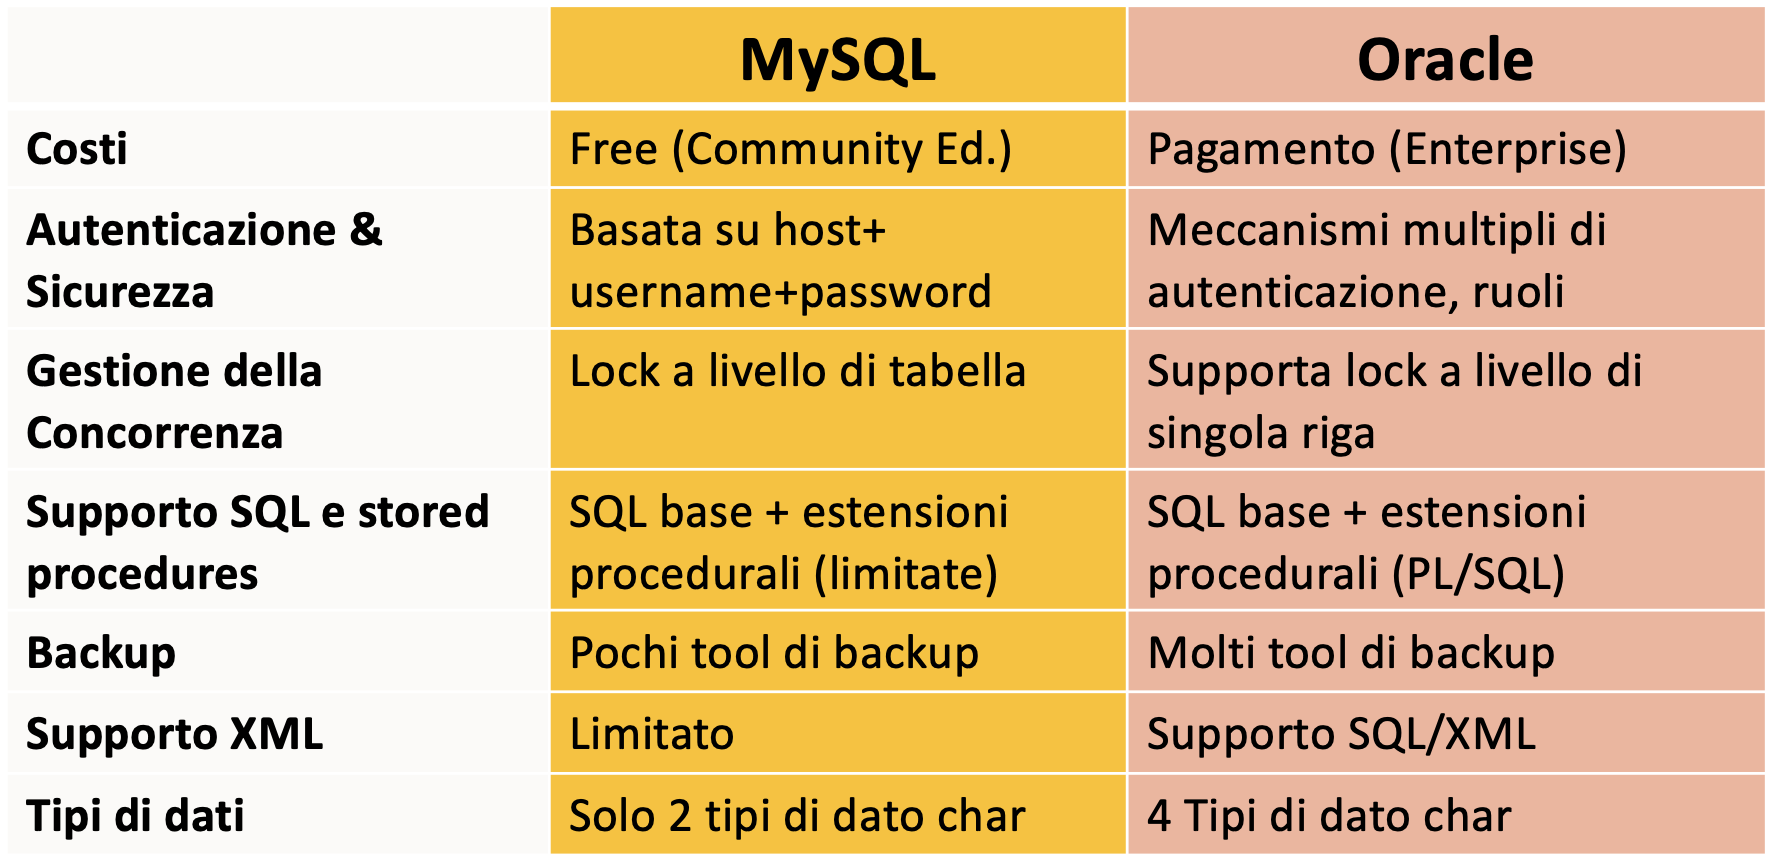
\includegraphics[width=1\textwidth]{foto 1.png}
\end{center}
\end{document}